% English draft based on sections/13_conclusion_ja.tex
\section{Conclusion: What Remains Open}

\noindent\textbf{Scope of the account.} The conclusions below retain local definitions, conditional formal discussion, and proposed architecture as distinct contributions. They do not establish universal cognitive nonclosure, necessary external stopping, generated stopping layers, field/network identity, or mobility/error equivalence. Historical operations remain conceptual readings or hypotheses. Future quantification and stopping-functional work remain open; their absence is not filled by the summary or by the figures. The negative implementation, ethical, and phenomenal scope is unchanged.


This paper has described the dynamics of intelligence, not prescribed its implementation. Its claims concern how inference, logs, stopping layers, thresholds, and external reference fields move.

\subsection{Three Logical Lines}

\textbf{First: non-closure and external stopping.} In the historical local-state model, the inference operator $F$ is discussed under strict-increase and fixed-region premises. Relating $L_F$ to all cognitive stopping remains open; externalization is a separate proposal.

\textbf{Second: threshold mobility.} The distinction between responsive and silent worlds is threshold-dependent. $\mu_\theta$ is the capacity to move the threshold and reorganize the movement region.

\textbf{Third: three-layer dynamics.} Traces of $L_F$ are related to $L_R$ as a log-reference role. The motion of $L_R$ under $H_{ij}$ is hypothesized to support $L_E$. Cooperation of $L_F$, $L_R$, and $L_E$ remains an architecture proposal; trace naming does not establish retention or emergence.

The current architectural contribution is the distinction between a tracked support, its scoped trace or quasi-stable retention role, and its temporary scaffold regime, with Unknown and descriptor-only ownness preserved. The preceding emergence language retains its historical proposal, not a proof supplied by this account. Later developmental quantification, stopping-functional work, and Part I proposals remain future or unimplemented work, not consequences newly established by the role descriptions.

\subsection{VED Principle in the Intelligence Layer}

VED's vocabulary of motion arising from difference motivates a role comparison here. The proposed account of intelligence does not establish the same principle as a typed cognitive mechanism.

\begin{figure}[H]
\centering
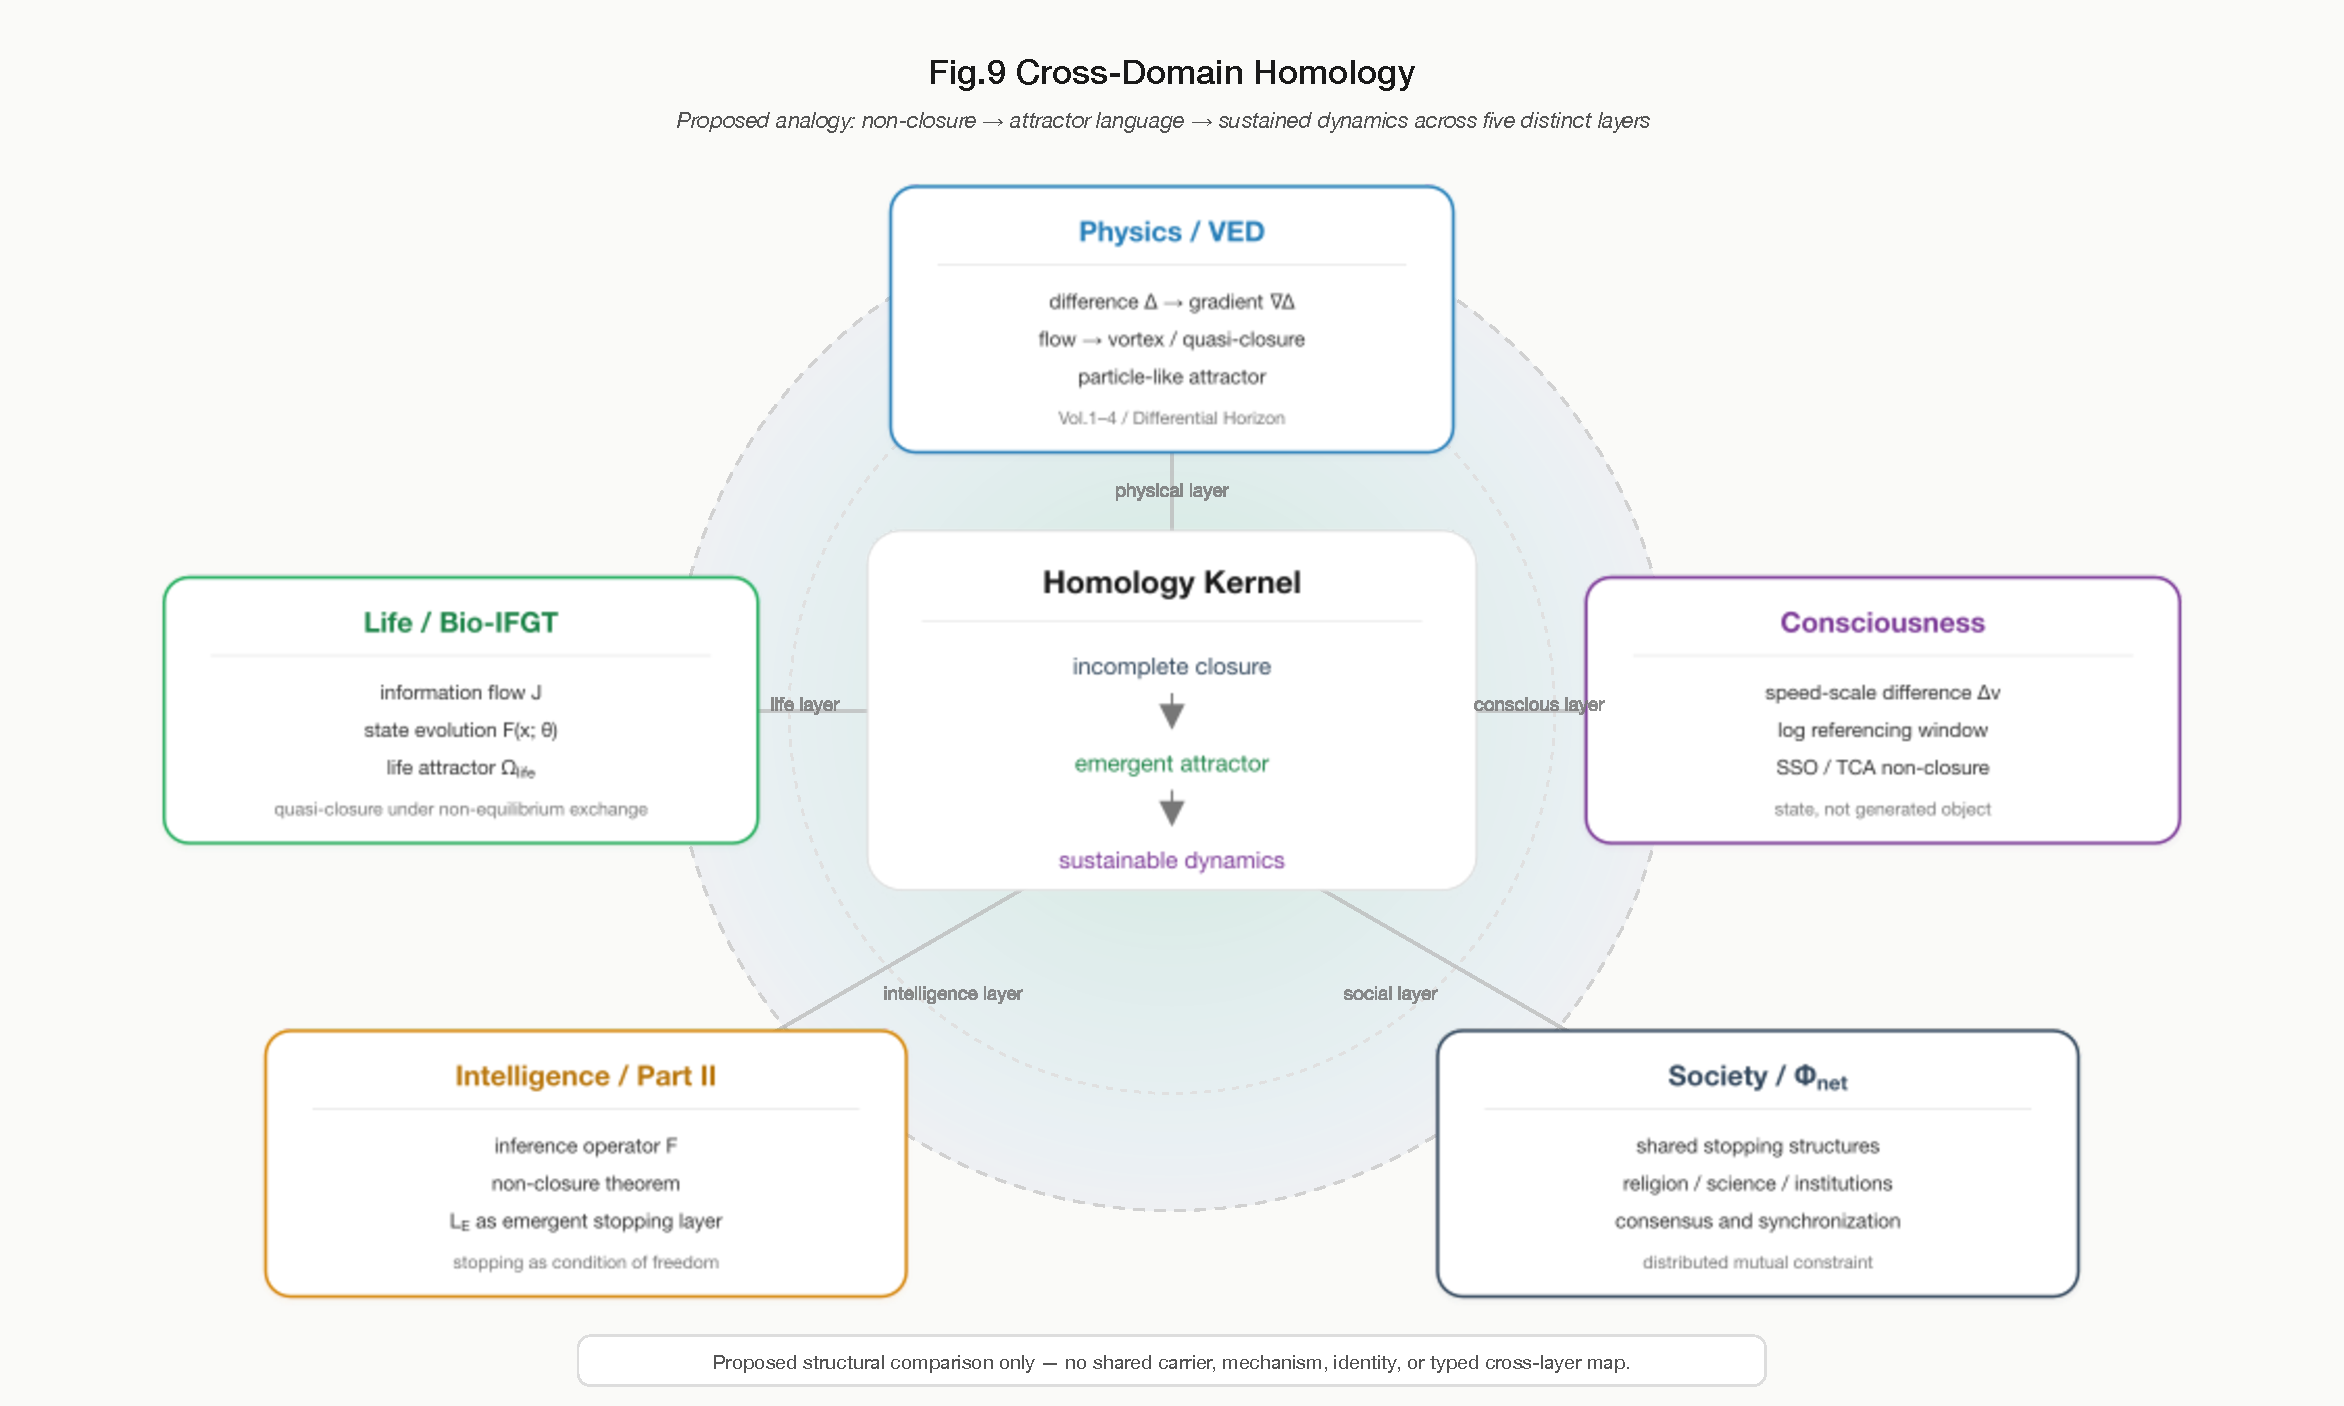
\includegraphics[width=\linewidth]{fig9_cross_domain_homology.pdf}
\caption{A proposed cross-domain comparison of incomplete closure, attractor-like organization, and sustained dynamics.}
\label{fig:part2-cross-domain-homology}
\figurenote{The central sequence is used as a comparison scaffold; each domain card contains source-local objects and claims.}{The figure proposes a formal-role analogy. It does not establish a common carrier, mechanism, identity, or typed cross-domain translation.}
\end{figure}

\subsection{Open Questions}

Several questions are intentionally left open. The meaning of understanding is passed to the philosophical layer. AI implementation and governance are outside this paper's descriptive scope. Quantifying the developmental degree of $L_E$ remains a future task. Formalizing a stopping functional analogous to closure energy is also left for later work.

\subsection{Final Statement}

The model describes nonclosed motion and proposed stopping roles. Its persistence is hypothesized to involve externally related, revisable stopping; neither persistence in general nor independent existence and detection of that stopping is established.

Sapiens-like intelligence adds endogenous $\mu_\theta$: the ability to move the region in which stopping can be installed. The proposed links among mobility, revision, error, and persistence retain separate formal and empirical burdens.

Theory ends here. The questions do not.

\bigskip
